\section{浮力}\label{sec:6-1}

船能够浮在水面上,是因为浸在水里的船身受到水的向上托的力。
木块能够浮在水面上,是因为浸在水里的木块受到水的向上托的力。
浸在水中的物体受到的水的向上托的力叫做\textbf{浮力}。
实际上,不仅浮在水面上的物体受到浮力,浸没在水中的物体也受到浮力。
这可以用下面的实验来证明。把一个金属块挂在弹簧秤上,读出弹簧秤的读数。
然后把金属块浸没在水中,可以看到,弹簧秤的读数减小了(图 \ref{fig:6-1})。弹簧秤前后两次读数的差就是金属块受到的浮力。
从井里提水,觉得水桶浸没在水里时比离开水面以后轻,就是因为水桶在水里时受到水的浮力。
从水里救溺水的人时,用不大的力就能把人的头部托出水面,也是因为人在水里受到水的浮力。

\begin{figure}[htbp]
    \centering
    \begin{minipage}{7cm}
    \centering
    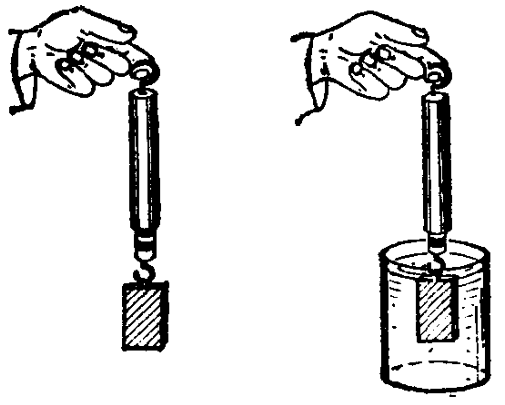
\includegraphics[width=7cm]{../pic/czwl1-ch6-1}
    \caption{}\label{fig:6-1}
    \end{minipage}
    \qquad
    \begin{minipage}{7cm}
    \centering
    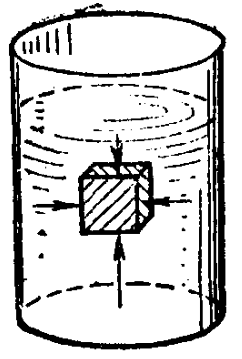
\includegraphics[width=3.5cm]{../pic/czwl1-ch6-2}
    \caption{}\label{fig:6-2}
    \end{minipage}
\end{figure}

不但水有浮力,煤油、酒精、水银等所有的液体,对浸在它们里面的物体都有浮力。

浮力是怎样产生的呢?这可以用图 \ref{fig:6-2} 来说明。

假设有一个正方体完全浸没在水里,我们知道,液体对它里面的一切物体都有压强,而且压强随深度的增加而增大。
所以正方体的前后、左右、上下六个面都受到水的压力。由于左右两个侧面的对应部分在水中的深度相同,
所受到的水的压强大小相等,所以作用在左右两侧面上的压力大小相等,方向相反,彼此平衡。
同样,作用在前后两侧面上的压力也彼此平衡。但是上下两面由于在水中的深度不同,受到的压强也不相等。
上面的压强小,下面的压强大,所以下面受到的向上的压力比上面受到的向下的压力大。
\CJKunderwave{水对物体向上和向下的压力的差就是水对物体的浮力}。
因此,\CJKunderwave{浮力总是竖直向上的}。

\CJKunderwave{物体在气体中也受到浮力}。氢气球脱手后会上升,就是因为受到空气对它的浮力。

